\documentclass[]{article}
\usepackage{graphicx}
\usepackage{lmodern}
\usepackage{amssymb,amsmath}
\usepackage{ifxetex,ifluatex}
\usepackage{fixltx2e} % provides \textsubscript
\ifnum 0\ifxetex 1\fi\ifluatex 1\fi=0 % if pdftex
  \usepackage[T1]{fontenc}
  \usepackage[utf8]{inputenc}
\else % if luatex or xelatex
  \ifxetex
    \usepackage{mathspec}
  \else
    \usepackage{fontspec}
  \fi
  \defaultfontfeatures{Ligatures=TeX,Scale=MatchLowercase}
\fi
% use upquote if available, for straight quotes in verbatim environments
\IfFileExists{upquote.sty}{\usepackage{upquote}}{}
% use microtype if available
\IfFileExists{microtype.sty}{%
\usepackage{microtype}
\UseMicrotypeSet[protrusion]{basicmath} % disable protrusion for tt fonts
}{}
\usepackage{hyperref}
\hypersetup{unicode=true,
            pdftitle={Homework 1},
            pdfborder={0 0 0},
            breaklinks=true}
\urlstyle{same}  % don't use monospace font for urls
\IfFileExists{parskip.sty}{%
\usepackage{parskip}
}{% else
\setlength{\parindent}{0pt}
\setlength{\parskip}{6pt plus 2pt minus 1pt}
}
\setlength{\emergencystretch}{3em}  % prevent overfull lines
\providecommand{\tightlist}{%
  \setlength{\itemsep}{0pt}\setlength{\parskip}{0pt}}
\setcounter{secnumdepth}{0}
% Redefines (sub)paragraphs to behave more like sections
\ifx\paragraph\undefined\else
\let\oldparagraph\paragraph
\renewcommand{\paragraph}[1]{\oldparagraph{#1}\mbox{}}
\fi
\ifx\subparagraph\undefined\else
\let\oldsubparagraph\subparagraph
\renewcommand{\subparagraph}[1]{\oldsubparagraph{#1}\mbox{}}
\fi

\title{Homework 1}

\usepackage{geometry}
\geometry{letterpaper,textwidth=350pt,textheight=680pt,tmargin=60pt,
            left=72pt,footskip=24pt,headsep=18pt,headheight=14pt}
\usepackage{amsmath}
\usepackage{amssymb}
\usepackage{textcase}
\usepackage{soul}

\newcommand{\mat}[1]{\boldsymbol{#1}}
\renewcommand{\vec}[1]{\boldsymbol{\mathrm{#1}}}
\newcommand{\vecalt}[1]{\boldsymbol{#1}}

\newcommand{\conj}[1]{\overline{#1}}

\newcommand{\normof}[1]{\|#1\|}
\newcommand{\onormof}[2]{\|#1\|_{#2}}

\newcommand{\itr}[2]{#1^{(#2)}}
\newcommand{\itn}[1]{^{(#1)}}

\newcommand{\eps}{\varepsilon}
\newcommand{\kron}{\otimes}

\DeclareMathOperator{\diag}{diag}
\DeclareMathOperator{\trace}{trace}
\DeclareMathOperator{\tvec}{vec}

\newcommand{\prob}{\mathbb{P}}
\newcommand{\probof}[1]{\prob\left\{ #1 \right\}}

\newcommand{\pmat}[1]{\begin{pmatrix} #1 \end{pmatrix}}
\newcommand{\bmat}[1]{\begin{bmatrix} #1 \end{bmatrix}}
\newcommand{\spmat}[1]{\left(\begin{smallmatrix} #1 \end{smallmatrix}\right)}
\newcommand{\sbmat}[1]{\left[\begin{smallmatrix} #1 \end{smallmatrix}\right]}

\newcommand{\RR}{\mathbb{R}}
\newcommand{\CC}{\mathbb{C}}

\providecommand{\eye}{\mat{I}}
\providecommand{\mA}{\ensuremath{\mat{A}}}
\providecommand{\mB}{\ensuremath{\mat{B}}}
\providecommand{\mC}{\ensuremath{\mat{C}}}
\providecommand{\mD}{\ensuremath{\mat{D}}}
\providecommand{\mE}{\ensuremath{\mat{E}}}
\providecommand{\mF}{\ensuremath{\mat{F}}}
\providecommand{\mG}{\ensuremath{\mat{G}}}
\providecommand{\mH}{\ensuremath{\mat{H}}}
\providecommand{\mI}{\ensuremath{\mat{I}}}
\providecommand{\mJ}{\ensuremath{\mat{J}}}
\providecommand{\mK}{\ensuremath{\mat{K}}}
\providecommand{\mL}{\ensuremath{\mat{L}}}
\providecommand{\mM}{\ensuremath{\mat{M}}}
\providecommand{\mN}{\ensuremath{\mat{N}}}
\providecommand{\mO}{\ensuremath{\mat{O}}}
\providecommand{\mP}{\ensuremath{\mat{P}}}
\providecommand{\mQ}{\ensuremath{\mat{Q}}}
\providecommand{\mR}{\ensuremath{\mat{R}}}
\providecommand{\mS}{\ensuremath{\mat{S}}}
\providecommand{\mT}{\ensuremath{\mat{T}}}
\providecommand{\mU}{\ensuremath{\mat{U}}}
\providecommand{\mV}{\ensuremath{\mat{V}}}
\providecommand{\mW}{\ensuremath{\mat{W}}}
\providecommand{\mX}{\ensuremath{\mat{X}}}
\providecommand{\mY}{\ensuremath{\mat{Y}}}
\providecommand{\mZ}{\ensuremath{\mat{Z}}}
\providecommand{\mLambda}{\ensuremath{\mat{\Lambda}}}
\providecommand{\mPbar}{\bar{\mP}}

\providecommand{\ones}{\vec{e}}
\providecommand{\va}{\ensuremath{\vec{a}}}
\providecommand{\vb}{\ensuremath{\vec{b}}}
\providecommand{\vc}{\ensuremath{\vec{c}}}
\providecommand{\vd}{\ensuremath{\vec{d}}}
\providecommand{\ve}{\ensuremath{\vec{e}}}
\providecommand{\vf}{\ensuremath{\vec{f}}}
\providecommand{\vg}{\ensuremath{\vec{g}}}
\providecommand{\vh}{\ensuremath{\vec{h}}}
\providecommand{\vi}{\ensuremath{\vec{i}}}
\providecommand{\vj}{\ensuremath{\vec{j}}}
\providecommand{\vk}{\ensuremath{\vec{k}}}
\providecommand{\vl}{\ensuremath{\vec{l}}}
\providecommand{\vm}{\ensuremath{\vec{l}}}
\providecommand{\vn}{\ensuremath{\vec{n}}}
\providecommand{\vo}{\ensuremath{\vec{o}}}
\providecommand{\vp}{\ensuremath{\vec{p}}}
\providecommand{\vq}{\ensuremath{\vec{q}}}
\providecommand{\vr}{\ensuremath{\vec{r}}}
\providecommand{\vs}{\ensuremath{\vec{s}}}
\providecommand{\vt}{\ensuremath{\vec{t}}}
\providecommand{\vu}{\ensuremath{\vec{u}}}
\providecommand{\vv}{\ensuremath{\vec{v}}}
\providecommand{\vw}{\ensuremath{\vec{w}}}
\providecommand{\vx}{\ensuremath{\vec{x}}}
\providecommand{\vy}{\ensuremath{\vec{y}}}
\providecommand{\vz}{\ensuremath{\vec{z}}}
\providecommand{\vpi}{\ensuremath{\vecalt{\pi}}}

\sodef\allcapsspacing{\upshape}{0.15em}{0.65em}{0.6em}%

\makeatletter
\def\maketitle{%
\par
\hrule height 0.75pt\vspace{1ex}
\par\noindent
\begin{minipage}{0.5\textwidth}
\scshape
purdue university $\cdot$ cs 51400 \\
numerical analysis
\end{minipage}
\begin{minipage}{0.5\textwidth}
\raggedleft
\MakeTextUppercase{\allcapsspacing{\@title}}\\[0.2ex]
\textit{\@author}\\[0.2ex]
\textit{\@date}
\end{minipage}
\par\vspace{1ex}
\hrule height 1pt
\vspace{2ex}
\par
}
\makeatother

\author{David F. Gleich}
\title{Lecture Notes}
% auto generate a title
% \AtBeginDocument{\maketitle}

\title{Homework}

% indent !!
\setlength{\parindent}{2em}

\begin{document}
\maketitle

Name : Tian Qiu\\
PUID: 00265 35063

\section{Homework 1}\label{homework-1}

\subsection{Problem 1: G \& C, Chapter 1, Problem 2 (10
points)}\label{problem-1-g-c-chapter-1-problem-2-10-points}


(a)
if x = 3, \\
After one step p(2) = .5  \&  p(4) = .5\\
After two steps\\
\indent	p(1) = .5 * p(2) + .5*p(0)  = .25\\
\indent	p(3) = 1 - .25 - .25  = .5\\
\indent	p(5) = .5 * p(4)  = .25\\
	
\noindent(b)
Reach the bar first:\\
\indent	x = 1\\
Reach home first:\\
\indent	x = 4\\
Becasue x = 1 is the closest step to bar and x = 2 is the cloest step to the home.


\subsection{Problem 2: A simple economy (10
points)}\label{problem-2-a-simple-economy-10-points}


\begin{enumerate}
\def\labelenumi{\arabic{enumi}.}
\item
\indent Total Demand = [8+1+1+8+7, 29, 21] = [25, 29, 21]\\
\indent total crude oil industry = [0, 100, 50]\\
\indent total refining industry = [232, 0, 174]\\
\indent total utility industry = [21, 126, 0]\\

\item
profit of the crude oil industry is $ =  [0, 100, 50] * [4, 3, 2]^{T} = 400$

\end{enumerate}

\subsection{Problem 3: Adding acceleration to the raptor problem (15
points)}\label{problem-3-adding-acceleration-to-the-raptor-problem-15-points}


\begin{enumerate}
\def\labelenumi{\arabic{enumi}.}
\item
Assumption and model:\\
a). Runner will always runin the same speed after acceleration when the time goes on.\\
c). Constant acceleration rate
b). The runner will just go in the straight line\\\\
$ v $ end speed\\
$ t $ end time\\
acceleretion a = $ \frac{v}{t} $
distance s = $ \dfrac{t * v}{2} $ = $ \dfrac{a * t^{2}}{2} $
\\\\\\

\item
 Immediately begins running at 12 meters-per-second: \\
 \indent distance s = 12 * t = 12t meters\\
 Accelerate to 12 meters-per-second:\\
 \indent distance s = .5 * 2  * 6 + 12 * (t-6) = 12t -72 + 6 = 12t - 66 meters \\
 
 The distance difference between these two types is 66 meters
\end{enumerate}

\subsection{Problem 4: Search engines (15
points)}\label{problem-4-search-engines-15-points}

\begin{enumerate}
\def\labelenumi{\arabic{enumi}.}
\item
$$
\begin{matrix}
1 & 0 & 0 \\
1 & 1 & 0 \\
1 & 0 & 1 \\
1 & 1 & 1
\end{matrix} 
$$

\item
  $$
  \begin{matrix}
  0 & 0 & 0 & 1 & 0 \\
  1 & 0 & 0 & 0 & 0 \\
  1 & 0 & 0 & 0 & 0 \\
  0 & 1 & 1 & 0 & 1 \\
  0 & 0 & 1 & 0 & 0
  \end{matrix} 
  $$
  
\item
    $$
    \begin{matrix}
    0.03 \\
    0.03\\
    0.03\\
    0.88\\
    0.03 
    \end{matrix} 
    $$
\end{enumerate}




\subsection{Problem 5: Intro to Julia (15
points)}\label{problem-5-intro-to-julia-15-points}

\begin{enumerate}
\def\labelenumi{\arabic{enumi}.}
\item
  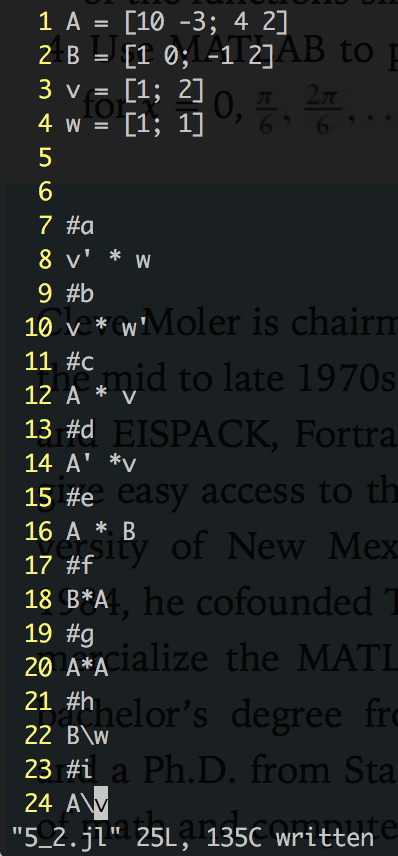
\includegraphics{5_1}
\item
 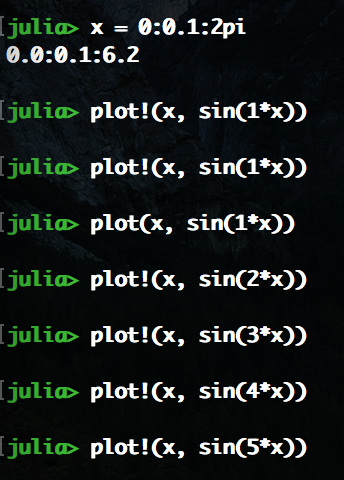
\includegraphics{5_2}\\
 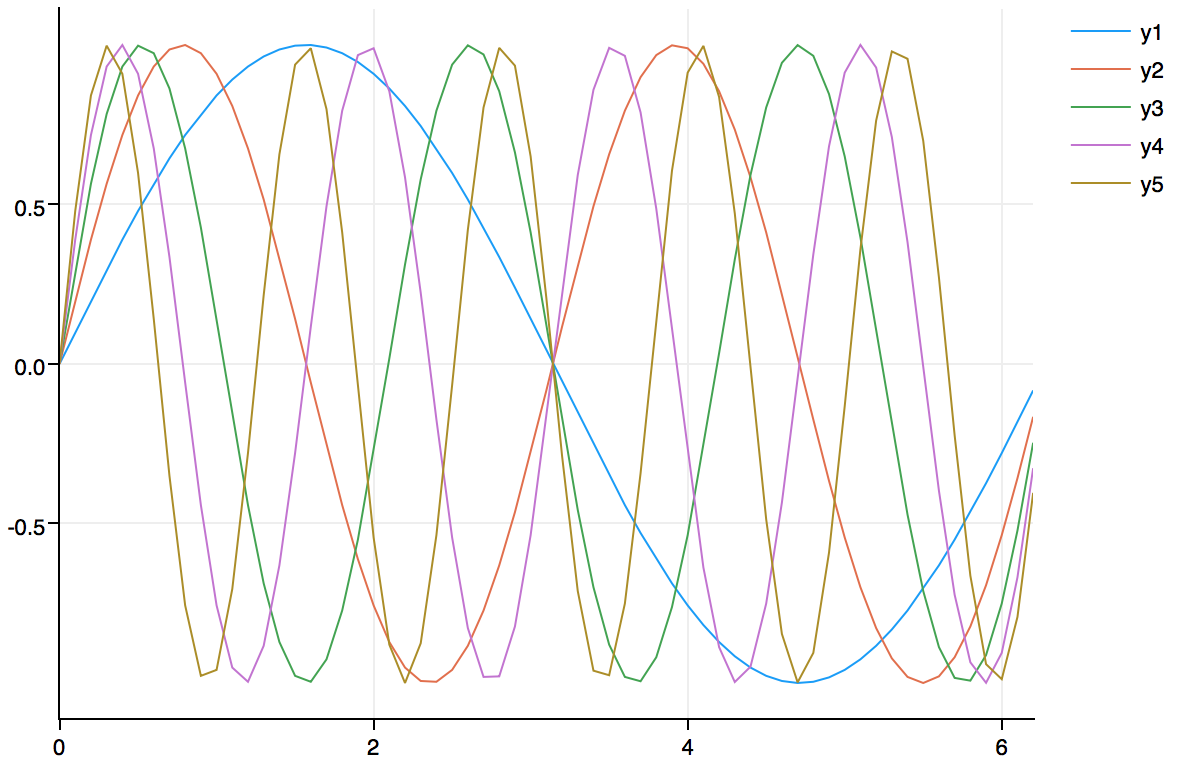
\includegraphics[scale = 0.8]{5_2_1}
\item
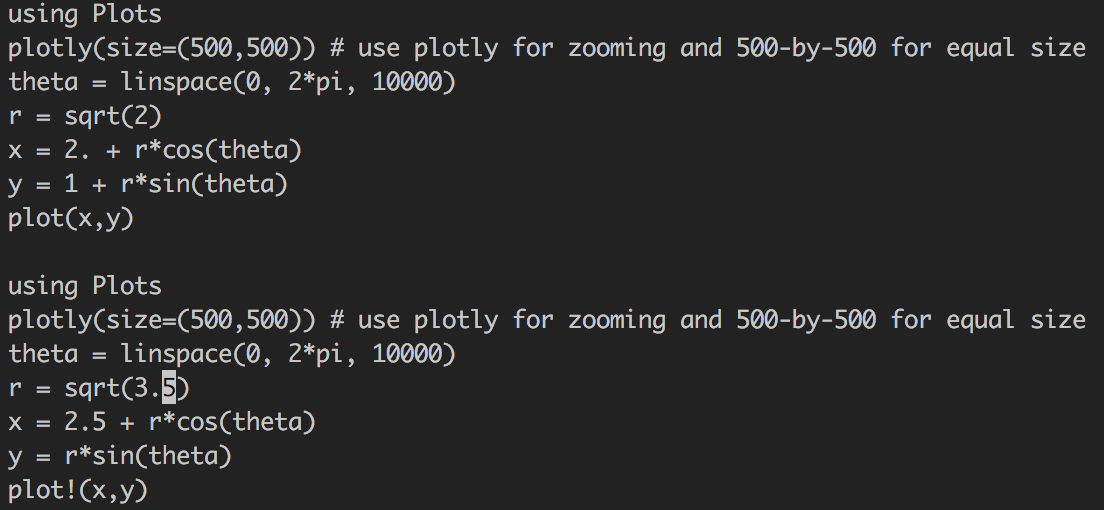
\includegraphics{5_3}
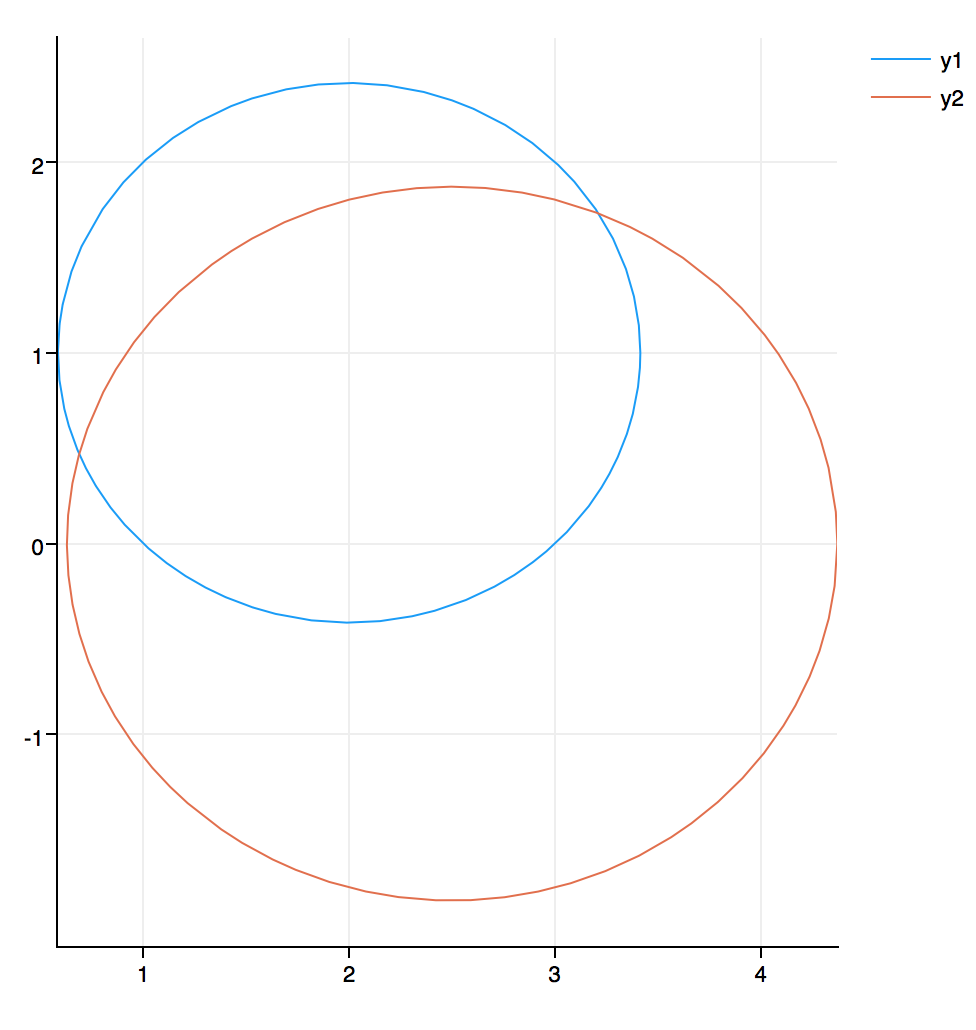
\includegraphics[scale=0.8]{5_3_1}

\end{enumerate}






\subsection{Problem 6: Drawing the Julia set (25
points)}\label{problem-6-drawing-the-julia-set-25-points}

2. 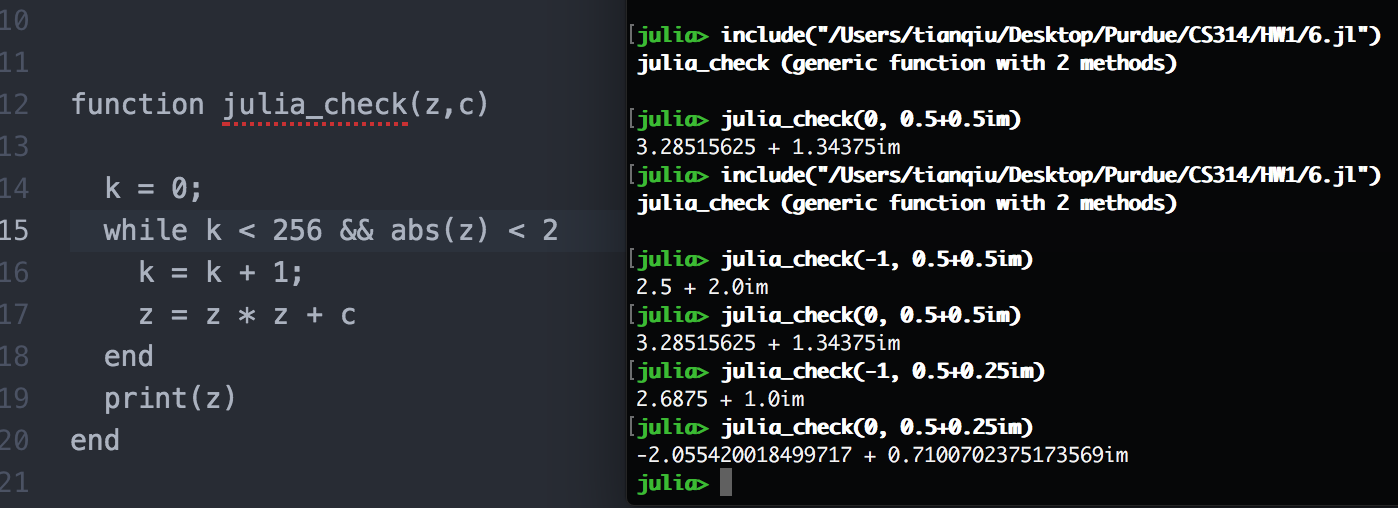
\includegraphics[scale=0.6]{6_1}

3. 
\includegraphics[scale=0.5]{6_4}\\
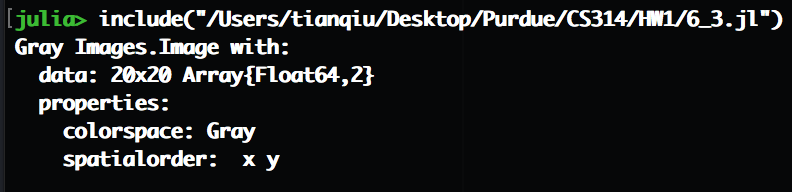
\includegraphics[scale=0.8]{6_2}\\
4. 
\includegraphics[scale=0.5]{6_5}
  Which one do you like better?\\
  
  I like the image when c=0.5+0.5i, because it is more spiral and more symmtrical, which is more beautiful.
  














\subsection{Problem 7: Fun with Julia (5
points)}\label{problem-7-fun-with-julia-5-points}


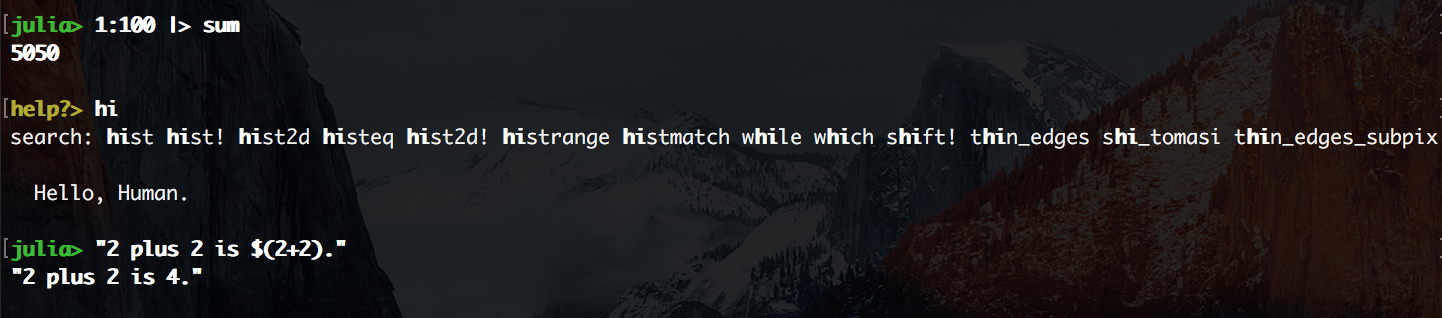
\includegraphics[scale=0.8]{7}
see or hear:\\

1. sum is the function \\

2. ? is going into help session \\

3. \$ sign can add value in string\\


\end{document}
